% !TEX root = ../main.tex
\documentclass[../main.tex]{subfiles}

\begin{document}
\section{iPXE scripting}

\subsection{Scripting overview}

The iPXE firmware comes with a built-in scripting language that allows for a wide range of customizations.
This language resembles a shell scripting language, but is more limited in its capabilities.
The primary operations that can be performed are:

\begin{itemize}
  \item \textbf{Variable assignment}: Variables can be set and read, and can be used to store configuration values
  \item \textbf{Control flow}: iPXE supports basic control flow statement based on the \texttt{goto} command and labels
  \item \textbf{Configuration}: iPXE scripting API allows for configuration of network interfaces with both static and dynamic IP addresses
  \item \textbf{Certificate management}: iPXE scripting API allows for management of certificates and keys, this allows for secure communication with HTTPS servers and loading only trusted scripts
  \item \textbf{HTTP requests}: Scripting language supports making HTTP requests, although the usage is limited to downloading scripts and files
  \item \textbf{Basic user interaction via console}: iPXE scripting comes with a set of commands that allow basic I/O (Input and Output) operations via the console
\end{itemize}

Comments in iPXE scripting are prefixed with the \texttt{\#} character and are ignored by the interpreter.
It is important to start all iPXE scripts with a comment that contains the \texttt{\#!ipxe} string.
The hash character followed by an exclamation mark is called a shebang. It is used to indicate
how the file should be interpreted when executing this file.

By default, the iPXE interpreter will try to interpret any file
as a binary executable which will lead to crash in the pre boot environment which will lead to a system reboot.

\subsection{Variables}

The iPXE script primarily serves to set up the boot process, and it utilizes variables to store the configuration.
Variables are stored as arrays of bytes \cite{ipxe_settings_types_docs}, when working with variables for most cases it is sufficient to treat them as strings.
All variables are accessible globally and can be read and written to at any time.
The detailed list of variable types is not documented in the official documentation \cite{ipxe}, but can be found in the source code \cite{ipxe_settings_types}.


The scripting environment comes with a set of predefined variables that hold the current configuration of the system.
For example, the \texttt{net0/ip} variable holds the IP address of the first network interface. Setting
this variable will change the IP address of the first network interface.
The variables can be accessed using the \texttt{set} and \texttt{isset} commands.
The \texttt{set} command takes two arguments, the first argument is the name of the variable and the second argument is the value that the variable will be set to.
The \texttt{isset} command takes one argument, the name of the variable, and returns 1 if the variable is set and 0 otherwise.
For accessing the value of a variable, the \texttt{\$\{variable\_name\}} syntax is used.

\begin{listing}[H]
  \textfile{modern-network-booting/code/variable_operations.ipxe}
  \caption{Basic variable operations in iPXE scripts}
\end{listing}

To display the value of a variable, either the \texttt{echo} or \texttt{show} commands can be used.
The \texttt{echo} command will print the value that was passed to it, while the \texttt{show} command
will use the passed value as the name of the variable and print its value alongside variable type.

\begin{listing}[H]
  \textfile{modern-network-booting/code/variable_types.ipxe}
  \caption{Setting and displaying variable types in iPXE scripts, the commands are executed in the iPXE shell}
\end{listing}


Although using string values for variables might suffice, there are situations where it becomes beneficial to incorporate additional validation to ensure that the value aligns with the correct type.
The type of variable can be explicitly provided by suffixing the value with the colon character (\texttt{:}) and the type of the variable.
When using a given variable for a value of another variable, the resulting type of the variable will be the same as the type of the variable that is currently being set, this
is demonstrated in listing \ref{code:variable_types_when_assigning}.

\begin{listing}[H]
  \textfile{modern-network-booting/code/variable_types_when_assigning.ipxe}
  \caption{How types of variables are inferred when assigning values to variables}
  \label{code:variable_types_when_assigning}
\end{listing}

Some commands require the value to be of a specific type, most notable the increment (\texttt{inc}) and decrement (\texttt{dec}) commands, this is demonstrated in listing \ref{code:increment_type_safety}.

\begin{listing}[H]
  \textfile{modern-network-booting/code/increment_type_safety.ipxe}
  \caption{Increment command interactions with values of different types}
  \label{code:increment_type_safety}
\end{listing}

\subsection{Control flow}
All ipxe scripts are executed sequentially, line by line.
Each line is broken down into commands and arguments and executed in the defined order.

To define multiple commands in the same line one of the following commands separators must be used.

\begin{itemize}
  \item \texttt{;}    - Executes the next command regardless of the result of the previous command
  \item \texttt{\&\&} - Executes the next command only if the previous command was successful
  \item \texttt{||}   - Executes the next command only if the previous command failed
\end{itemize}

\begin{listing}[H]
  \textfile{modern-network-booting/code/control_flow_example.ipxe}
  \caption{Basic control flow operations in iPXE scripts}
\end{listing}

Combining the usage of \texttt{\&\&} and \texttt{||} allows for basic
if-else logic to be implemented in the iPXE scripting language.
As these operators rely on the return value of the previous command,
they can be used for basic error handling. Return value of 0 indicates success,
while any other value indicates failure.

To define more complex control flow, the \texttt{goto} command can be used.
The \texttt{goto} command takes one argument, the name of the label to jump to.
Labels are defined using the \texttt{:} character followed by the name of the label.
The \texttt{goto} command can be used to implement loops and conditional statements.

\begin{listing}[H]
  \textfile{modern-network-booting/code/goto_example.ipxe}
  \caption{Infinite loop implemented using goto command}
\end{listing}

Any kind of control flow can be implemented by combining the \texttt{goto} command with variables.

\begin{listing}[H]
  \textfile{modern-network-booting/code/for_loop_example.ipxe}
  \caption{"For loop" construct implemented in iPXE scripts}
  \label{code:for_loop_example}
\end{listing}

Listing \ref{code:for_loop_example} demonstrates how a "for loop" can be implemented in iPXE scripts. As shown in the example this kind of loop can be used to
iterate over network interfaces and perform operations on them.

\subsection{Configuring boot process}

\subsubsection{DHCP configuration}

In order to use network communication in iPXE scripts, the network interface must be configured.
For most use cases, the \texttt{dhcp} command can be used to configure the network interface with a dynamic IP address.
The \texttt{dhcp} command takes one argument which determinate the network interface to configure.
If no argument is provided, the configuration will be tried on all network interfaces.
Additionaly the \texttt{dhcp} command can be passed the \texttt{--timeout} parameter which will set the timeout for the DHCP request.
As stated by the official documentation \cite{ipxe_dhcp_vs_ifconfig} there is no difference between using the \texttt{dhcp} command and the \texttt{ifconf}.

\begin{listing}[H]
  \textfile{modern-network-booting/code/dhcp_configuration.ipxe}
  \caption{Configuring network interface using the \texttt{dhcp} command}
  \label{code:dhcp_configuration}
\end{listing}

Listing \ref{code:dhcp_configuration} demonstrates how the \texttt{dhcp} command can be used to configure the network interface.
The \texttt{dhcp} command will be executed in a loop until the network interface is configured with a dynamic IP address.

\subsubsection{Static IP configuration}

When the network interface need to be configured with a static IP address, the \texttt{set} command can be used,
to configure the \texttt{ip}, \texttt{netmask} and \texttt{gateway} variables.


Additionaly network interfaces have to be first opened using the \texttt{ifopen} command.
All network interfaces are closed by default. As pointed out in the documentation opening too much network interfaces can lead to memory exhaustion \cite{ipxe_opening_interfaces}.

\begin{listing}[H]
  \textfile{modern-network-booting/code/static_ip_configuration.ipxe}
  \caption{Configuring \texttt{net0} network interface with a static IP address}
  \label{code:static_ip_configuration}
\end{listing}

\subsection{Booting kernel image}

To boot a kernel image, the \texttt{kernel} command can be used to fetch and specify the kernel image to boot.
This command takes the URI of the kernel image as the first argument and the arguments to pass to the kernel as the second argument.
As pointed out in the documentation notes section \cite{ipxe_kernel_command}, \texttt{imgselect} and \texttt{imgload} are aliases for the \texttt{kernel} command.

Booting only a kernel image will result in a kernel panic, as kernel image does not contain any root filesystem.
To attach a root filesystem the \texttt{initramfs} disk image is used. Its purpose is to provide a temporary root filesystem that will be used to boot the system.
After kernel boots, it mounts this filesystem under  "\texttt{/}" and then executes "\texttt{/init}" binary which is responsible for mounting the real root filesystem from persistent storage like a hard drive \cite{initramfs_purpose}.

\begin{listing}[H]
  \textfile{modern-network-booting/code/booting_sysrescue.ipxe}
  \caption{Booting the SystemRescue\cite{sysrescuecd} OS}
  \label{code:ipxe_sysrescue_boot}
\end{listing}

Listing \ref{code:ipxe_sysrescue_boot} demonstrates how the \texttt{kernel} command can be used to boot the SystemRescue OS.
Kernel binary image alongside initramfs images are downloaded from HTTP server after \texttt{dhcp} network configuration is performed.
Many distributions require additional kernel parameters to be passed to the kernel, SystemRescue OS requires
memory file system to be loaded which is located in the \texttt{airootfs.sfs} file \cite{systemrescue_airootfs_pxe}.
This is done by passing the base URI and directory containing the \texttt{airootfs.sfs} file as arguments to the \texttt{kernel} command line.


To boot different distributions, refer to the documentation specific to each distribution to identify the necessary kernel parameters.
The \texttt{Netboot.xyz} project \cite{netbootxyz} offers a diverse collection of iPXE scripts designed for booting different distributions.
This resource can serve as a guide for booting distributions that may lack dedicated documentation for PXE booting.

\subsection{Interacting with the user}

\subsubsection{Menu}

The most common form of user interaction found in iPXE scripts is the menu.
The commands that are used to create and manage menus are \texttt{menu}, \texttt{item} and \texttt{choose}.

The \texttt{menu} command takes one optional argument, the name of the menu, executing this command will create a new menu which can be later referred to by its name in other commands.
If no argument is provided, the default menu will be created. The default menu is referenced in other commands by omitting the menu parameter.


To add item to the menu, the \texttt{item} command is used. It takes two arguments, the first argument is the name of the entry and the second value is the displayed label of the entry.
The difference between the name and the label are that the name is used to reference the entry in other commands, while the label is the text that will be displayed to the user.
For example, the name of the entry can be "\texttt{sysrescue}" while the label would be "\texttt{SystemRescue}". The user would only see the label, while
the result that returned by the \texttt{choose} command would be the "\texttt{sysrescue}" name.

In addition to the name and label, \texttt{--name} parameter can be used to specify the name of the menu that the entry belongs to. And the \texttt{--key}
parameter can be used to specify a shortcut key that upon pressing will select the entry.


To display the menu to the user, the \texttt{choose} command is used.
It takes one argument which is the name of a variable to which the result of the menu will be assigned.
Additionaly it takes the \texttt{--menu} parameter which specifies the name of the menu to display.
The \texttt{choose} command will display the menu to the user and wait for the user to select an entry.

\begin{listing}[H]
  \textfile{modern-network-booting/code/ipxe_simple_menu.ipxe}
  \caption{Simple iPXE menu for choosing OS to boot}
  \label{code:ipxe_simple_menu}
\end{listing}

\begin{figure}[H]
  \centering
  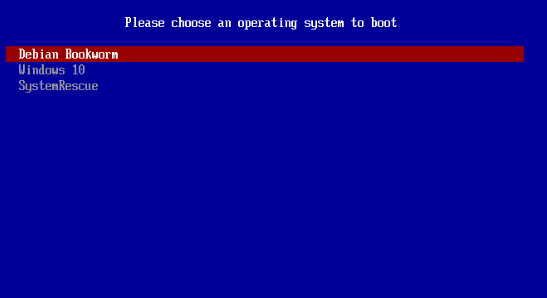
\includegraphics[width=\textwidth]{ipxe/simple_menu.png}
  \caption{Menu shown to the user using script from listing \ref{code:ipxe_simple_menu}}
  \label{fig:ipxe_simple_menu}
\end{figure}

After user selects an entry in the menu shown in figure \ref{fig:ipxe_simple_menu}, the \texttt{choose} command will write the name of the selected entry to the \texttt{os} variable
as shown in listing \ref{code:ipxe_simple_menu_result}.

\begin{listing}[H]
  \begin{textcode}
    iPXE> show os
    os:string = windows10
  \end{textcode}
  \caption{Contents of the \texttt{os} variable after selecting the \texttt{windows10} entry in the menu shown in figure \ref{fig:ipxe_simple_menu}}
  \label{code:ipxe_simple_menu_result}
\end{listing}

\subsubsection{Customizing the menu appearance}

The menu appearance can be customized using the \texttt{console} command.
This command allows settings background image, resolution and margins of the menu.
Additionally, the \texttt{color} command can be used to change the color foreground and background colors of the printed text.

\begin{listing}[H]
  \textfile{modern-network-booting/code/ipxe_custom_menu.ipxe}
  \caption{Customizing the menu appearance}
  \label{code:ipxe_custom_menu}
\end{listing}

The prompt command used in listing \ref{code:ipxe_custom_menu} is used to delay the execution of the script until the user presses a key.
This command is useful to ensure that the user has enough time to read the menu before it disappears.

\begin{figure}[H]
  \centering
  
\includegraphics[width=\textwidth]{ipxe/customized_menu.png}
  \caption{Customized menu shown to the user using script from listing \ref{code:ipxe_custom_menu}}
  \label{fig:ipxe_custom_menu}
\end{figure}

\subsection{Embedding scripts in the iPXE firmware image}

When the unmodified iPXE binary is executed, it prompts the user to press \texttt{Ctrl+B} to enter the iPXE shell. Following a brief delay, an automatic boot is initiated.

\begin{figure}[H]
  \centering
  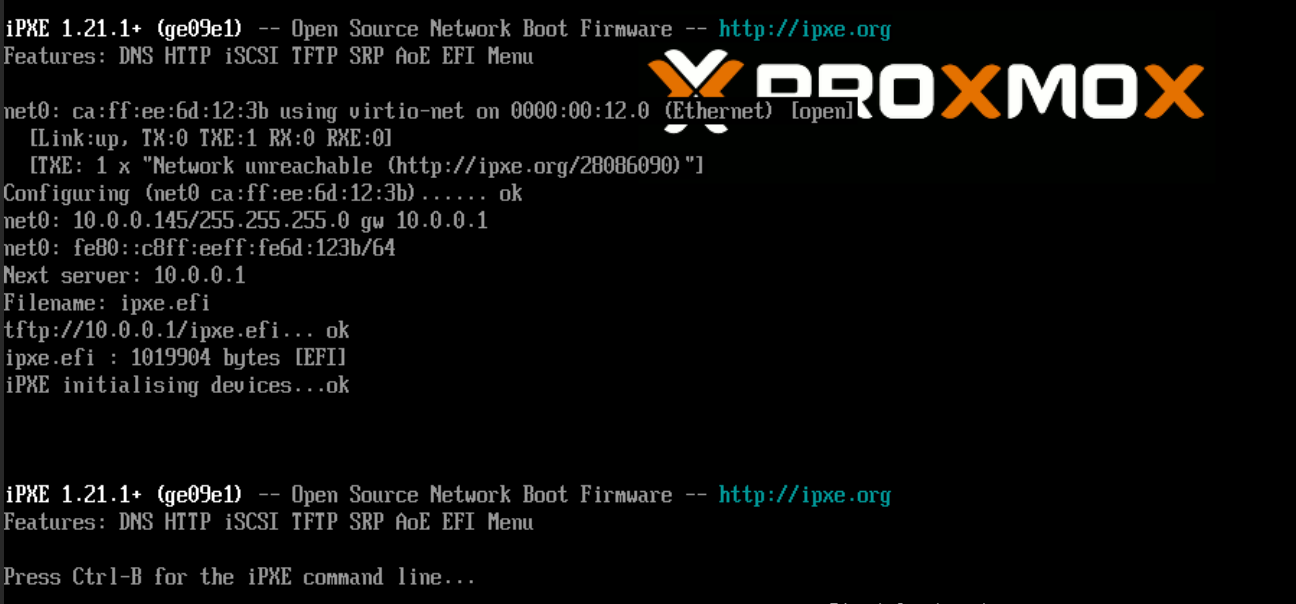
\includegraphics[width=\textwidth]{ipxe/default_boot.png}
  \caption{Default boot behavior of the iPXE firmware}
\end{figure}

During this automated boot process, the \texttt{next\_server} and \texttt{filename} DHCP options are used to determine the location of the script to execute.
Although this behavior is anticipated when the iPXE firmware is intended as a PXE substitute, it poses issues when the iPXE firmware has already been loaded from the default NIC PXE firmware utilizing these variables.

In these cases the iPXE firmware will attempt to load once again the same script that was used to load the iPXE firmware. This will result in an infinite loop of loading the same script over and over again.
The loop will hang when all the available memory is exhausted and the system will freeze.

To customize the boot behavior of the iPXE firmware, an iPXE script can be embedded in the iPXE image. It will be executed automatically when the iPXE firmware is loaded.
This script will replace the default boot behavior of the iPXE firmware, which includes the prompt for the user to press \texttt{Ctrl+B} to enter the iPXE shell.
To embed a script in the iPXE firmware, the \texttt{EMBED} variable must be supplied to the \texttt{make} command when compiling the iPXE firmware.
This variable must contain the path to the script that will be embedded in the iPXE firmware.

\begin{listing}[H]
  \begin{bashcode}
    make -j $(nproc --all) EMBED=script.ipxe bin-x86_64-efi/ipxe.efi
  \end{bashcode}
  \caption{Compiling the iPXE firmware with an embedded script}
\end{listing}

\end{document}